\documentclass[a4paper,5pt]{amsbook}
%%%%%%%%%%%%%%%%%%%%%%%%%%%%%%%%%%%%%%%%%%%%%%%%%%%%%%%%%%%%%%%%%%%%%

\usepackage{booktabs}
\usepackage{graphicx}
\usepackage{multicol}
\usepackage{textcomp}
\usepackage{systeme}
\usepackage{amssymb}
\usepackage[]{amsmath}
\usepackage{subcaption}
\usepackage[inline]{enumitem}
\usepackage{gensymb}
\usepackage[utf8]{inputenc}

%%%%%%%%%%%%%%%%%%%%%%%%%%%%%%%%%%%%%%%%%%%%%%%%%%%%%%%%%%%%%%

\newcommand{\sen}{\,\mbox{sen}\,}
\newcommand{\tg}{\,\mbox{tg}\,}
\newcommand{\cosec}{\,\mbox{cosec}\,}
\newcommand{\cotg}{\,\mbox{cotg}\,}
\newcommand{\tr}{\,\mbox{tr}\,}
\newcommand{\ds}{\displaystyle}

%%%%%%%%%%%%%%%%%%%%%%%%%%%%%%%%%%%%%%%%%%%%%%%%%%%%%%%%%%%%%%%%%%%%%%%%

\setlength{\textwidth}{16cm} \setlength{\topmargin}{-1.3cm}
\setlength{\textheight}{30cm}
\setlength{\leftmargin}{1.2cm} \setlength{\rightmargin}{1.2cm}
\setlength{\oddsidemargin}{0cm}\setlength{\evensidemargin}{0cm}

%%%%%%%%%%%%%%%%%%%%%%%%%%%%%%%%%%%%%%%%%%%%%%%%%%%%%%%%%%%%%%%%%%%%%%%%

% \renewcommand{\baselinestretch}{1.6}
% \renewcommand{\thefootnote}{\fnsymbol{footnote}}
% \renewcommand{\theequation}{\thesection.\arabic{equation}}
% \setlength{\voffset}{-50pt}
% \numberwithin{equation}{chapter}

%%%%%%%%%%%%%%%%%%%%%%%%%%%%%%%%%%%%%%%%%%%%%%%%%%%%%%%%%%%%%%%%%%%%%%%

\begin{document}
\thispagestyle{empty}
\pagestyle{empty}
\begin{minipage}[h]{0.14\textwidth}
	
\includegraphics[scale=0.24]{../../ufgd.png}
\end{minipage}
\begin{minipage}[h]{\textwidth}
\begin{tabular}{c}
{{\bf UNIVERSIDADE FEDERAL DA GRANDE DOURADOS}}\\
{{\bf C\'{a}lculo Diferencial e Integral II --- Lista 3}}\\
{{\bf Prof.\ Adriano Barbosa}}\\
\end{tabular}
\vspace{-0.45cm}
%
\end{minipage}

%------------------------

\vspace{1cm}
%%%%%%%%%%%%%%%%%%%%%%%%%%%%%%%%   formulario  inicio  %%%%%%%%%%%%%%%%%%%%%%%%%%%%%%%%
\begin{enumerate}
	\vspace{0.5cm}
	\item Escreva as frações abaixo como soma de frações parciais:

		\vspace{0.3cm}
		\begin{enumerate*}
			\item $\displaystyle\frac{1+6x}{(4x-3)(2x+5)}$
			\hspace{0.5cm}
			\hspace{0.5cm}
			\item $\displaystyle\frac{10}{5x^2-2x^3}$
		\end{enumerate*}

	\vspace{0.5cm}
	\item Calcule as integrais abaixo:
		\begin{enumerate}
			\vspace{0.3cm}
			\item $\displaystyle\int\frac{x^4}{x-1}\ dx$
			\vspace{0.3cm}
			\item $\displaystyle\int\frac{5x+1}{(2x+1)(x-1)}\ dx$
			\vspace{0.3cm}
			\item $\displaystyle\int\frac{ax}{x^2-bx}\ dx$
			\vspace{0.3cm}
			\item $\displaystyle\int\frac{x^3+4}{x^2+4}\ dx$
			\vspace{0.3cm}
			\item $\displaystyle\int_0^1\frac{x^3+2x}{x^4+4x^2+3}\ dx$
			\vspace{0.3cm}
			\item $\displaystyle\int\frac{1}{\sqrt{x}-\sqrt[3]{x}}\ dx$, use a substituição $u=\sqrt[6]{x}$
			\vspace{0.3cm}
			\item $\displaystyle\int\frac{e^{2x}}{e^{2x}+3e^x+2}\ dx$
			\vspace{0.3cm}
			\item $\displaystyle\int_3^4\frac{x^3-2x^2-4}{x^3-2x^2}\ dx$
			\vspace{0.3cm}
			\item $\displaystyle\int_1^2\frac{4y^2-7y-12}{y(y+2)(y-3)}\ dy$
			\vspace{0.3cm}
			\item $\displaystyle\int\frac{dx}{x(x^2+4)^2}$
		\end{enumerate}

	\vspace{0.5cm}
	\item Calcule as áreas das regiões abaixo, onde $x\in[1,2]$:

		\begin{enumerate*}
			\item 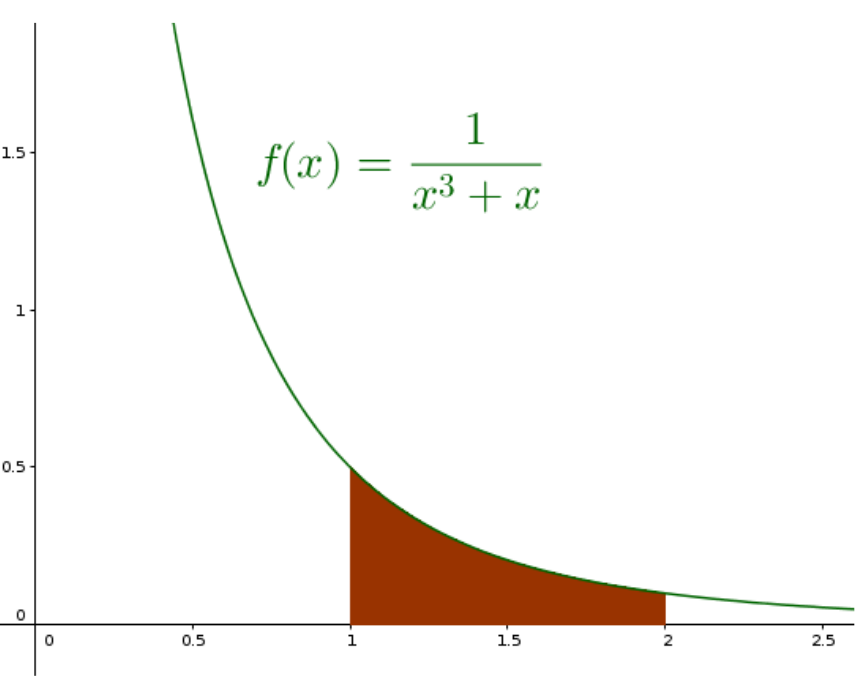
\includegraphics[width=5cm]{figs/lista03-3a.png}
			\hspace{1cm}
			\hspace{1cm}
			\item 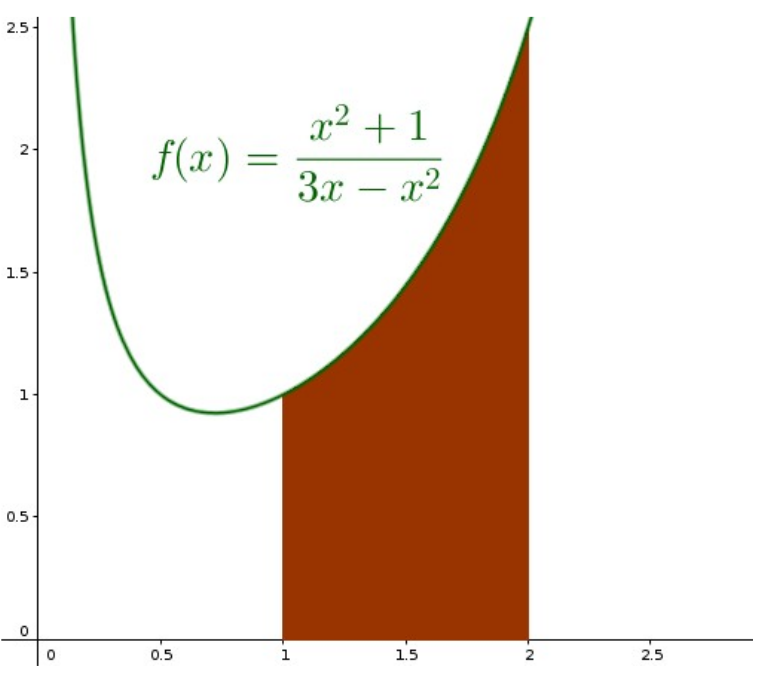
\includegraphics[width=5cm]{figs/lista03-3b.png}
		\end{enumerate*}
\end{enumerate}
\end{document}
